\subsection{Size of Type Vocabulary}\label{subsec:size-of-type-vocabulary}

Since we define our task as node (token) classification, we feed our transformer output into a classifier linear head.
Therefore, our type vocabulary is limited.
Because of the computational resources constraints, we limit it to one thousand types.

\begin{figure*}[t]
    \centering
    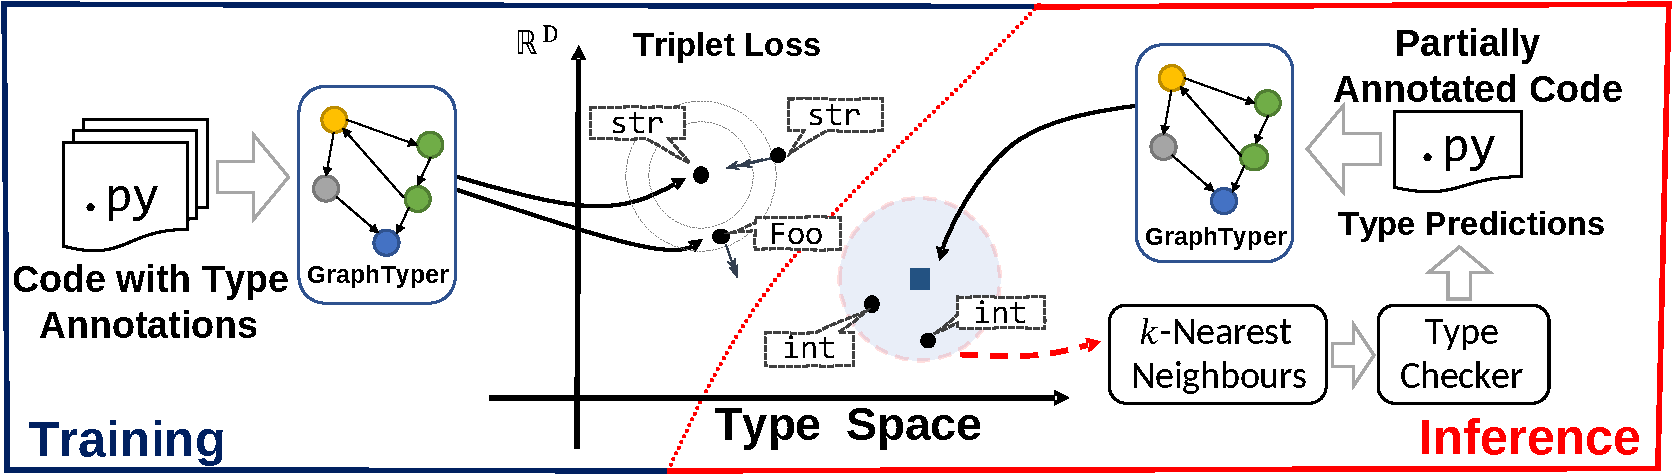
\includegraphics[width=0.75\textwidth]{figures/dsl.pdf}
    \caption{Solution to the problem using Deep Similarity Learning~\parencite{allamanis2020typilus}.}
    \label{fig:dsl}
\end{figure*}

This issue is addressable by formulating the task as Deep Similarity Learning Problem~\cite{chopra2005learning,liao2018tripletbased}.
In this way, the model will output vector representations of types that can be grouped into cluster of similar types.
After that, an algorithm such as KNN~\cite{knn} is used to transform vector representation into a probability of each type~\cite{allamanis2020typilus,mir_type4py_2021}.
Illustration for such an approach is depicted on Figure~\ref{fig:dsl}.
The approach follows the methodology described in Typilus paper~\cite{allamanis2020typilus}.

\subsection{Absence of Natural Language information}\label{subsec:absence-of-natural-language-information}

In our work, we use only categorical features of nodes and edges of code graph, e.g. AST node types and Python type annotations.
Therefore, it would be challenging to apply it directly for tasks such as code generation,
because the representation doesn't encode any information about variable names.

There are several approaches that would help address this issue.
Firstly, it is possible to use the model output as graph encoding that would be later fed into another model along with tokenized code~\cite{tipirneni_structcoder_2022}.
This approach could also address the issue from the previous Section~\ref{subsec:size-of-type-vocabulary}, since types would be treated as a set of text tokens~\cite{peng2023generative}.
Secondly, it is possible to use neural networks to infer variables' names from the context they are used in~\cite{bavishi2018context2name}.
